\documentclass[12pt]{article}
\usepackage{amsmath}
\usepackage{amsfonts}
\usepackage{geometry}
\usepackage{graphicx}
\usepackage{setspace}
\usepackage{parskip}
\usepackage{hyperref}
\usepackage{graphicx}
\usepackage{float}
\usepackage{booktabs}
\newcommand{\comm}[1]{def}

\geometry{a4paper, margin=1in}
\setstretch{1.2}

\title{\Huge Orderbook Delta price reaction research}
\author{}
\date{}





    


\begin{document}

\maketitle


\subsection*{Table of Contents}

\begin{itemize}
  \item Outlier Detection Using Mean and Standard Deviation (Z-Score Based Outlier Detection)
  \item Measuring Volatility After Price Outlier Detection
  \item Measuring avearge return after price outlier detection
  \item Combining Indicators
\end{itemize}



\subsection*{Orderbook Delta defenition}
The orderbook delta is calculate by the difference between the sum of the bid and ask orders at a certain depth.
Formular:
\begin{equation*}
  \Delta_{x\%} = \sum_{i=1}^{x\%} \Delta_{i}
\end{equation*}

\begin{itemize}
  \item $\Delta_{x\%}$ is the sum of the orderbook delta for the last $x\%$ of the orderbook.
  \item $\Delta_{i}$ is the orderbook delta for the $i$-th level of the orderbook.
\end{itemize}






\newpage

\section*{Outlier Detection Using Mean and Standard Deviation (Z-Score Based Outlier Detection)}


\subsection*{Normal Range}

What I want to test is how price reacts to anomalous orderbook delta movements, particularly in scenarios where unrealistic or clearly outlying values are detected. In cryptocurrency markets, such inefficiencies can be caused by various events, one example is liquidation
 events that interact with passive demand order stacked zones. During these events, the orderbook delta exhibits significant increases, providing a clear signal of market stress. This research will focus on understanding the relationship between rapid delta movements and how price reacts after these events.

\subsection*{My Hypothesis}

\begin{itemize}
  \item I expext realized volatility to increase after an outlier is detected. 
  \item I expext a return to the mean after a strong outlier is detected.
\end{itemize}



\subsection*{Normal Range}





\[
\mu(\Delta) \pm 2\sigma(\Delta)
\]

This means most data points (about 95\% if normally distributed) are expected to lie within this range.

\newpage

\subsection*{Outlier Condition}

A value is considered an outlier if:



\begin{equation}\label{eq: outlier_detection}
  \Delta < \mu(\Delta) - 2\sigma(\Delta) \quad \text{or} \quad \Delta > \mu(\Delta) + 2\sigma(\Delta)    
\end{equation}

This is a simple Z-score based outlier detection.

\begin{itemize}
  \item $\Delta$ - Orderbook Delta Depth with a certain depth I will test on: $\Delta_{1\%}$ $\Delta_{2.5\%}$ $\Delta_{5\%}$ from Coinbase (BTC/USD) 
  \item   This basically means we take a delta of the Bid and Ask orders which are in a range of x\% from the current price.
  \item $\mu(\Delta)$ — Mean of the last 1440 values of $\Delta$ before time $t$
  \item $\sigma(\Delta)$ - Standard deviation over the last 1440 $\Delta$ values before time $t$

\end{itemize}










\newpage


\subsection*{Idea behind}

\begin{itemize}
    \item This method assumes data is roughly normally distributed.
    \item Using $2\sigma$ captures approximately 95\% of data points under a normal distribution.
    \item You can adjust the multiplier (e.g., $3\sigma$) for stricter or looser thresholds.
\end{itemize}





\subsection*{Future Plans}

\begin{itemize}
    \item Test on more data
    \item use rolling windows (e.g. 1 day or 1 week) for local context.
    \item Compare sensitivity with +- 1.5$\sigma$ or +-2.5$\sigma$ $\rightarrow$ optimize for best results
\end{itemize}
















\newpage





\section*{Measuring Volatility After Price Outlier Detection}


\begin{equation}\label{eq:price_return}
    r_t = \frac{P_{t} - P_{t-1}}{P_{t-1}}
\end{equation}


\subsection*{Dictionary of Terms}

\begin{itemize}
    \item $P_t$  
      Asset price at time $t$.
    \item $r_t = \dfrac{P_t - P_{t-1}}{P_{t-1}}$  
      – 1-minute price return at time $t$.
    \item $\sigma^{\mathrm{(15)}}_{t}$  
      – Realized volatility: the standard deviation of the next 15 one-minute returns,
      
      

      
      \begin{equation}\label{eq:realized-vol}
        \sigma^{\mathrm{(15)}}_{t}
        = \sqrt{\frac{1}{14}\sum_{i=1}^{15}\bigl(r_{t+i}-\bar r_{t}\bigr)^{2}},
        \quad
        \bar r_{t} = \frac{1}{15}\sum_{i=1}^{15} r_{t+i}.
      \end{equation}
      



      aligned so that at time $t$ it measures volatility over $t+1$ to $t+15$.
\end{itemize}



\subsection*{In Python code}

\begin{verbatim}
import pandas as pd
df = pd.read_csv(file_path)
df.set_index('timestamp', inplace=True)
#Compute 1-min return of delta_5

df['r_t'] = df['price'].pct_change().fillna(0)


#compute rolling std of the future 15 min window

window = 15

#rolling on r_t, then shift forward so index t hold vol of t+1...t+15
df['future_vol_15] = (
    df['r_t']
    .rolling(window=window)
    .std()
    .shift(-window)
)
\end{verbatim}



\newpage

\subsection*{\textbf{Statistical evidence}}

Once an outlier is detected \eqref{eq: outlier_detection} inside of the Orderbook $\Delta$, we calculate the15-minute ahead realized volatility using Equation: \eqref{eq:realized-vol}




if a $\Delta_t$ values is flagged as an outlier \eqref{eq: outlier_detection}
we record
$$
\sigma^{(15)}_t
\;=\;
\sqrt{\frac{1}{14}\sum_{i=1}^{15}\bigl(r_{t+i}-\bar r_{t}\bigr)^{2}},
$$

We then form two samples over our full dataset which during this test includes 104 957 one minutes intervals of $P$ and Orderbook $\Delta$:


$$
\mathcal{S}_{\rm out} \;=\;\{\sigma^{(15)}_t : t\text{ is an outlier}\},
\quad
\mathcal{S}_{\rm non} \;=\;\{\sigma^{(15)}_t : t\text{ is not an outlier}\}.
$$


Sample mean results:
$$
\overline{\sigma}^{(15)}_{\rm out}
=0.0006244,
\qquad
\overline{\sigma}^{(15)}_{\rm non}
=0.0005138,
$$




This concludes an increase of $r_t$ of roughly 21.5\%


To check Statistical evidence

\begin{itemize}
  \item a two-sample *t*-test (unequal variances), which yields
  $$
    T=24.72,\quad p=4.79\times10^{-132},
  $$
  \item a Mann–Whitney *U*-test, which returns
  $$
    p=4.02\times10^{-157}.
  $$
\end{itemize}


\newpage

\section*{Optimising for best Z-Score thresold for outliers}

As state inside of \eqref{eq: outlier_detection} we use a Z-Score thresold of 2 to detect outliers. I now want to 
see if by any chance there is a better Thresold value  

To compare the outliers Volatility with the non outliers volatility I will use the following formular:

\begin{equation}\label{eq:vol_ratio}
U(z) =\frac{ \overline{\sigma}^{(15)}_{\rm out}}{\overline{\sigma}^{(15)}_{\rm non}}
\end{equation}


First I run an optimization for the thresholds of the Z-Score to find the best thresold value for the outliers on a 45 days dataset.
After that I compare the result with a 107880 minutes dataset. Where I also run an optimization for the thresholds of the Z-Score to find the best thresold value for the outliers.


Top 3 $z$-values with largest volatility uplift 69811-minutes sample

\begin{table}[H]
  \centering
  
  \label{tap:top3-z}
  \begin{tabular}{@{} c  r  r  r @{}}  
    \toprule
    $z$ & $N_{\rm out}$ & $U(z)$ (\%) & Mann–Whitney $p$ \\  
  \midrule
  3.8 & 221 &  +58.36 & $1.913\times10^{-51}$ \\  
  3.9 & 166 & +61.99 & $4.227\times10^{-41}$ \\  
  4.0 & 117 & +58.36 & $8.228\times10^{-28}$ \\ 
\bottomrule
\end{tabular}

\end{table}

Same $z$-values on extended dataset 107880-minutes sample

\begin{table}[H]
  \centering
  
  \label{tap:old-z-values-out-of-sample}
  \begin{tabular}{@{} c  r  r  r @{}}  
    \toprule
    $z$ & $N_{\rm out}$ & $U(z)$ (\%) & Mann–Whitney $p$ \\  
  \midrule
  3.8 & 644 & +51.73 & $2.549\times10^{-77}$ \\  
  3.9 & 561 & +53.28 & $6.150\times10^{-88}$ \\  
  4.0 & 479 & +50.90 & $5.517\times10^{-59}$ \\ 
\bottomrule
\end{tabular}

\end{table}





Top 3 $z$-values with largest volatility uplift 107880-minutes sample


\begin{table}[H]
  \centering
  
  \label{tap:top3-z-out-of-sample}
  \begin{tabular}{@{} c  r  r  r @{}}  
    \toprule
    $z$ & $N_{\rm out}$ & $U(z)$ (\%) & Mann–Whitney $p$ \\  
  \midrule
  4.8 & 214 & +65.10 & $6.475\times10^{-33}$ \\  
  4.9 & 197 & +66.81 & $3.693\times10^{-29}$ \\  
  5.0 & 181 & +70.53 & $6.599\times10^{-28}$ \\ 
\bottomrule
\end{tabular}

\end{table}












\newpage
\section*{Measuring avearge return after price outlier detection}




\subsection*{Formulars}
\begin{align}
\intertext{Once a $\Delta_t$ Outlier is detected we calculate the 15-min forward return of \underline{BTC/USD} price}
\mathrm{Ret}^{(15)}_t
\;=\;\frac{P_{t+15} - P_t}{P_t}
\tag{4}\\[1ex]
\intertext{We then differentiate between a bullish and a bearish outlier. Which is already defined \eqref{eq: outlier_detection}}
\overline{\mathrm{Ret}}^{(15)}_{\rm bull}
= \frac{1}{|\mathcal{T}_{\rm bull}|}
  \sum_{t\in\mathcal{T}_{\rm bull}} \mathrm{Ret}^{(15)}_t
\tag{7}\\[1ex]
\overline{\mathrm{Ret}}^{(15)}_{\rm bear}
= \frac{1}{|\mathcal{T}_{\rm bear}|}
  \sum_{t\in\mathcal{T}_{\rm bear}} \mathrm{Ret}^{(15)}_t
\tag{8}
\end{align}







\subsection*{Dictionary of Terms}

\begin{itemize}
  \item Price at a certain time: \space $P_t$
  \item 15-min forward return: \space $\mathrm{Ret}^{(15)}_t$
\end{itemize}





\begin{verbatim}
  #compute 15-min forward return of BTC/USD price
\end{verbatim}




\newpage


%complementation of indicators into a strategy
\section{Combining indicators for strategy}


\newpage
\section*{Underlying strategy Bias}

%underlying bias logic =     df['indiactor'] = (df['trend'] == 'Uptrend') & (df3['delta5'] > 0)
Every single parameter has to fight to be implemented into my strategy. To get some kind of filter since we are working with an asset which has clear trends and isn't stationary we need to do some trend identification.  
I'll call it the underlying bias. Some simple examples are for a bias are:
\begin{itemize}
  \item $\Delta_{5\%} < 0$ (more passive demand than supply)
  \item $EMA_{\text{n}} > P_t$ (EMA is an exponential average of $P_t-n$, $P-T$ is the price at time $t$)
  \item $EMA_{\text{n}} >EMA_{\text{x}}$ (Crossing of two EMAs with different time periods $n$ and $x$)
\end{itemize}

But I want to get some clear trend identification where we divide into the three different categories:


Ideas I want to test on:

\begin{itemize}
  \item Market Structure defenition (Higher Highs and Higher Lows)
  \item Realtive strenght index on Price and $\Delta_{x\%}$
  
  
\end{itemize}
\newpage
\section*{Finding an edge}
\subsection*{No clear path}
Finding an edge is a very hard task. There is no clear path to success. You kinda have to try by trail and error every error could be a step further but also a potential path into a dead end.
  

\newpage



Sources:
\href{https://trdr.io/}{TRDR} This platform allow you to use different kind of metrics on different Timeseries datasets (BTC/USD Price, orderbookdelta  and Open Interest






\newpage
\section{Comparison of Delta Indicators on 39,694-minute sample}

\begin{table}[h]
\begin{tabular}{cccc}
\hline
Period & $N_{signals}$ & $U(z)$ (\%) & T-statistic $p$ \\
\hline
\multicolumn{4}{l}{Delta2.5 Strategy ($N_{total}$ = 9,182)} \\
\hline
  $5m$ & $9,182$ & $+52.03$ & $1.851 \times 10^{-41}$ \\
  $60m$ & $9,182$ & $+55.94$ & $3.537 \times 10^{-4}$ \\
  $360m$ & $9,182$ & $+59.20$ & $12.524 \times 10^{0}$ \\
  \hline
  \multicolumn{4}{l}{Delta5 Strategy ($N_{total}$ = 12,234)} \\
  \hline
  $5m$ & $12,234$ & $+51.38$ & $3.382 \times 10^{-7}$ \\
  $60m$ & $12,234$ & $+53.44$ & $4.010 \times 10^{-1}$ \\
  $360m$ & $12,234$ & $+57.04$ & $13.617 \times 10^{0}$ \\
\hline
\end{tabular}
\caption{Comparison of Delta2.5 vs Delta5 strategies across different time periods}
\end{table}

\begin{itemize}
  \item $N_{signals}$ represents number of trading signals
  \item $U(z)$ represents positive return ratio
  \item T-statistic $p$ represents statistical significance
\end{itemize}





\newpage

\begin{figure}[H]
  \centering
  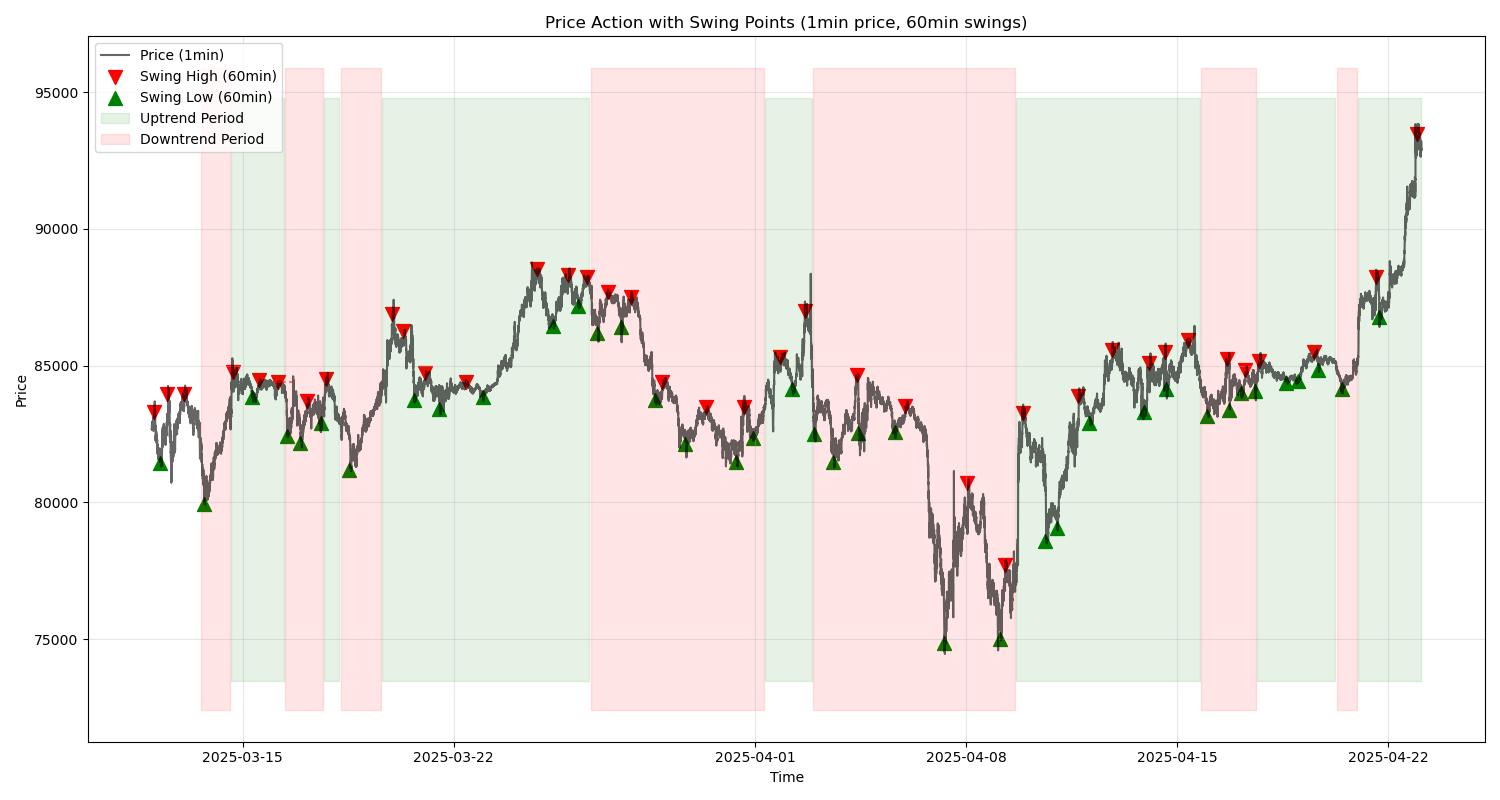
\includegraphics[width=\textwidth]{60min_swing_point_bias.png}
  \caption{1 min interval price with 60 min swing points and a $n$ value of 8 }
\end{figure}



\newpage
\section*{Swing Point Bias Visualization}

\begin{figure}[H]
    \centering
    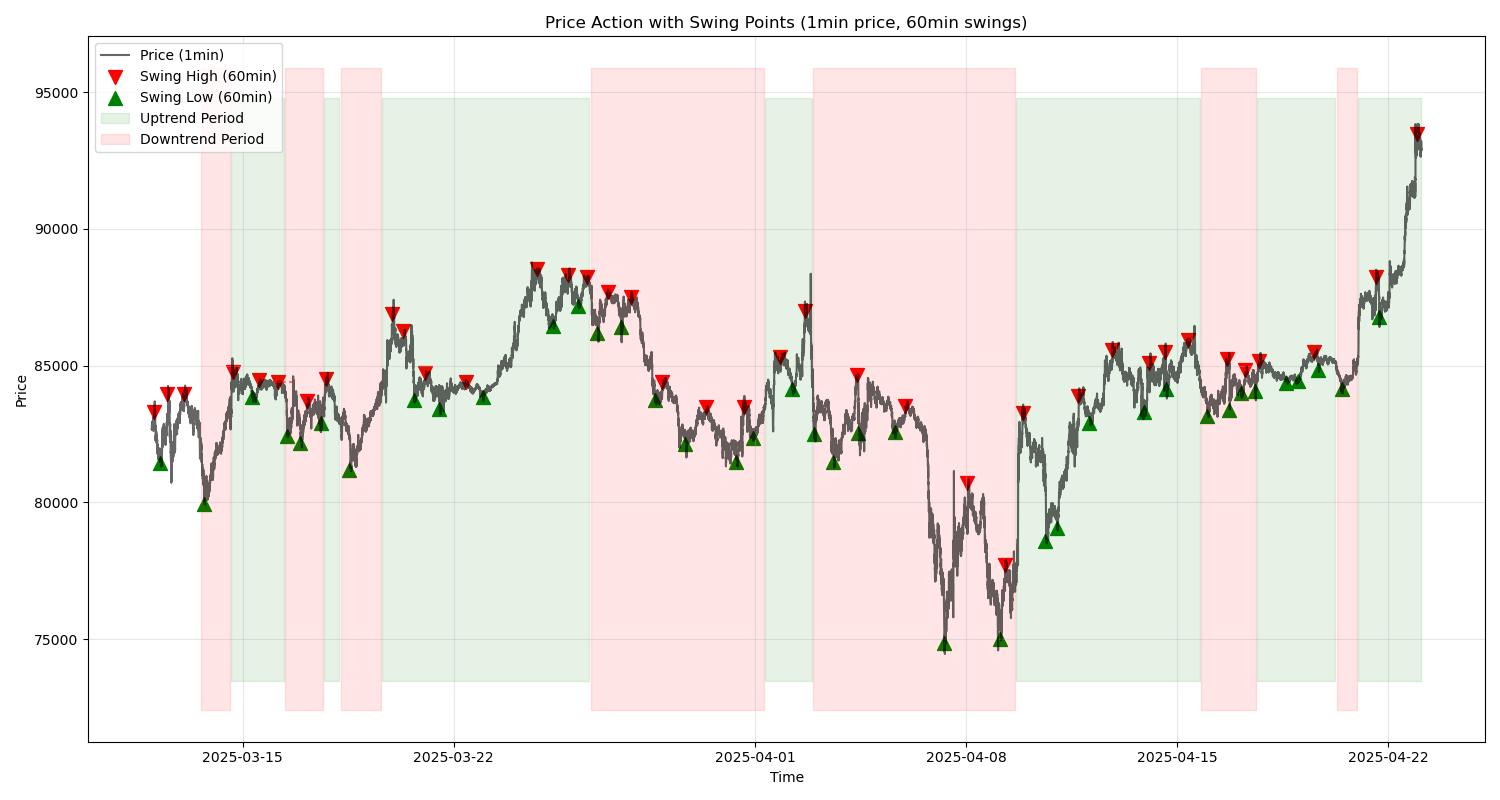
\includegraphics[width=\textwidth]{60min_swing_point_bias.png}
    \caption{Price Action with Swing Points (1min price, 60min swings) showing trend periods}
\end{figure}

% You might want to add a description or explanation here
This visualization demonstrates how swing points are identified on a 1-minute price chart using a 60-minute window for swing point detection. The green and red shaded areas represent uptrend and downtrend periods respectively, while red triangles mark swing highs and green triangles mark swing lows.

\newpage
\section*{Combining Indicators}
Here I visulised the swing points, the EMA spread and the 100 outliers with the highest Z-Score in the same plot.

\begin{figure}[H]
    \centering
    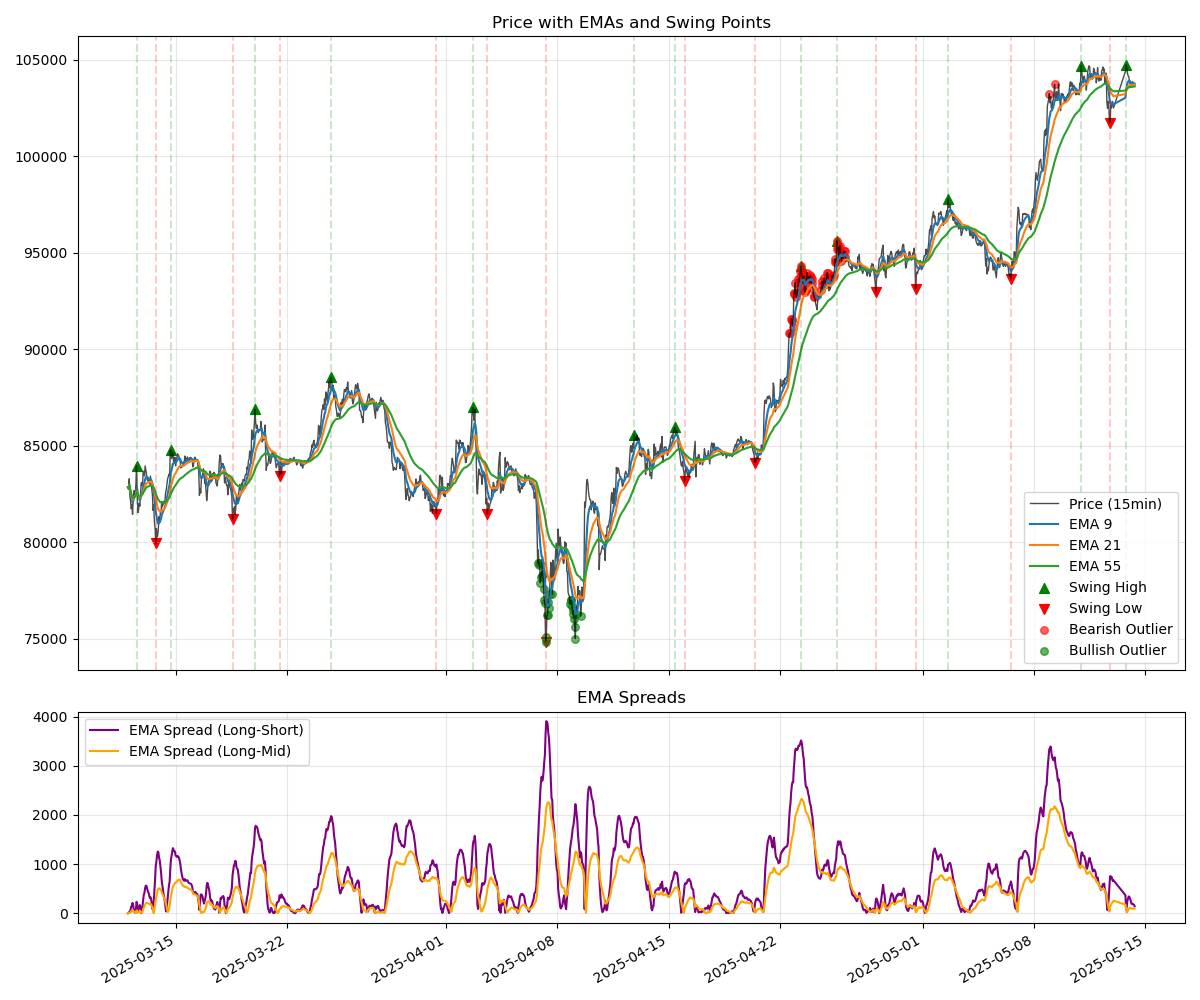
\includegraphics[width=\textwidth]{imgs/swingpoints_emaspread_priceOutliers.png}
    \caption{combined indicators png}
\end{figure}

\footnote{Chart made with Matplotlib and Seaborn}


\newpage
\section*{Mapping Orderbook delta EMA with standard deviation shifing}
\section*{Formulars}

\begin{equation}
  EMA_t = \alpha \cdot \Delta_t + (1 - \alpha) \cdot EMA_{t-1}
\end{equation}

Dictionary of Terms

\begin{itemize}
  \item $EMA_t$ - Exponential Moving Average at time $t$
  \item $\Delta_t$ - Orderbook delta at time $t$
  \item $\alpha$ - Smoothing factor 
  \item $\alpha = \frac{2}{n+1}$ where $n$ is the period of the EMA
  \item $\sigma(\Delta)$ - Standard deviation of the orderbook delta with a 
\end{itemize}

We'll now shift the EMA by the standard deviation of the orderbook delta 




\newpage
\section*{From outliers to strategy}
\subsection*{Progress description}
I had a pretty hard time going from developing a logic for the outliers of the Delta. Finding that volatility increases after outliers was a good first find which didn't take long to find. But finding some a defenition condtion is meet directional bias was very difficult. By directional bias I mean a price direction which is not random after some kind of condition. It was pretty clear from the begging on that the outliers by there selfe won't offer any kind of directional bias


An outlier is defined as:

\begin{itemize}
  \item \eqref{eq: outlier_detection}.
  $\Delta < \mu(\Delta) - 2\sigma(\Delta) \quad \text{or} \quad \Delta > \mu(\Delta) + 2\sigma(\Delta)    $
\end{itemize}


Then since we Bitcoin clearly is not a stationary asset I needed to find some kind of trend identification. I found that the swing points are a good indicator for this.
We determined a trend by using looking at swingpoints. A swing point is a local extrema of a certain period.

\subsection*{Where did I start my research}
\begin{verbatim}
  #compute swing points
  swing_points = swing_points(df['price'], period=n)

\end{verbatim}

Parameters of the swing\textunderscore points function:
\begin{itemize}
  \item $n$ is the lookback period
  \item $df['price']$ is the price column of the dataframe (Which is a timeseries)
  \item $P_t$ is a value of $df['price']$ at time $t$
\end{itemize}


We basically got through the time series dataset and look back $n$ $P_t$ values. The highest and lowest points inside of that specific lookback period are the swing points. After that we detetermine if price is making higher highs or lower lows. We check this by storeing the last swing points and wait till we are eighter making a higher high or a lower low.



\subsection*{Finding an edge}

\begin{figure}[H]
  \centering
  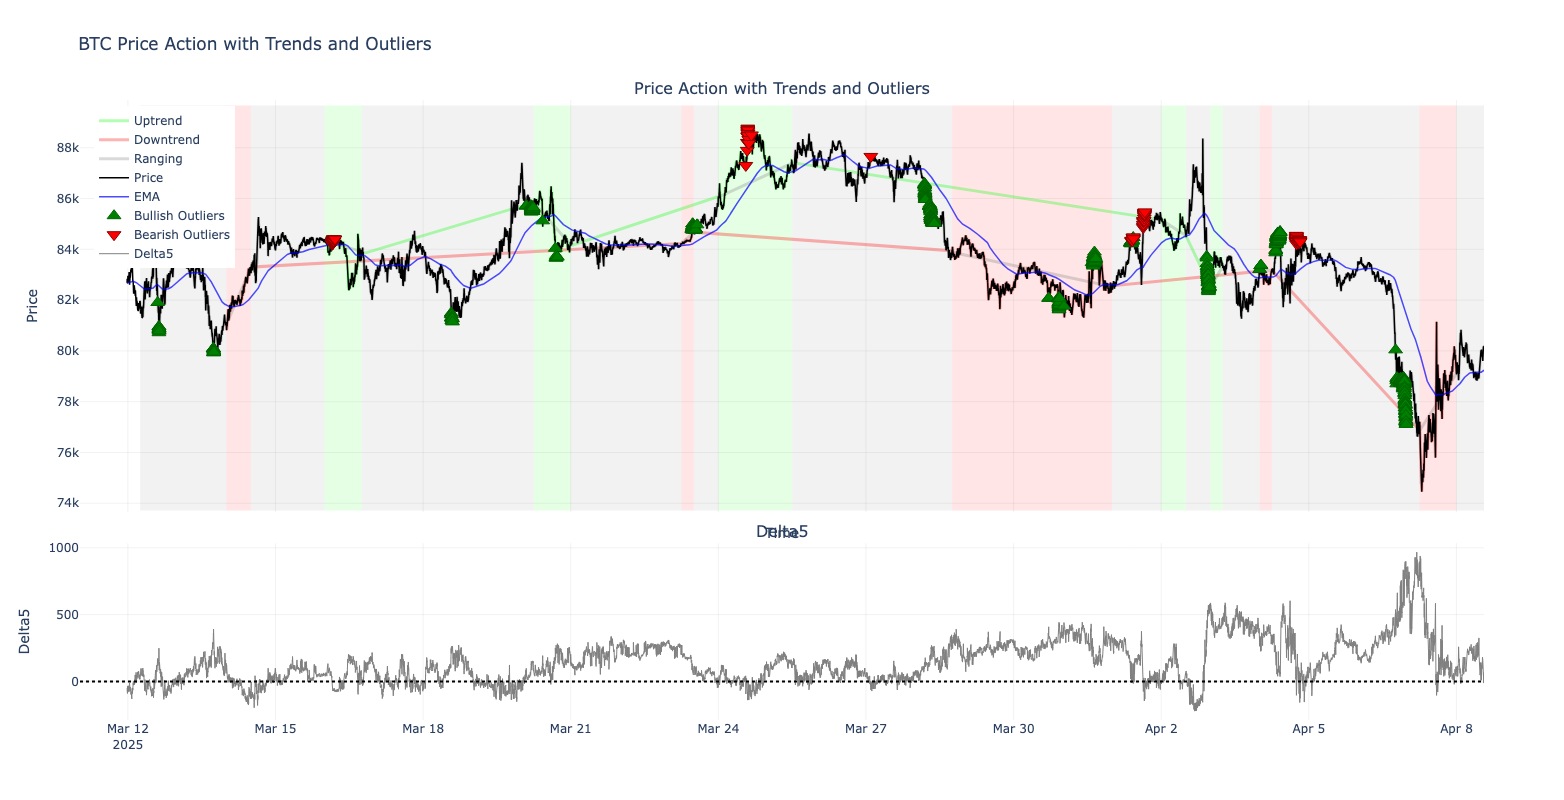
\includegraphics[width=\textwidth]{imgs/plotting_of_my_idea.png}
  \caption{Visualization of $\Delta_t$ outliers and swing points}
\end{figure}
\begin{figure}[H]
  \centering
  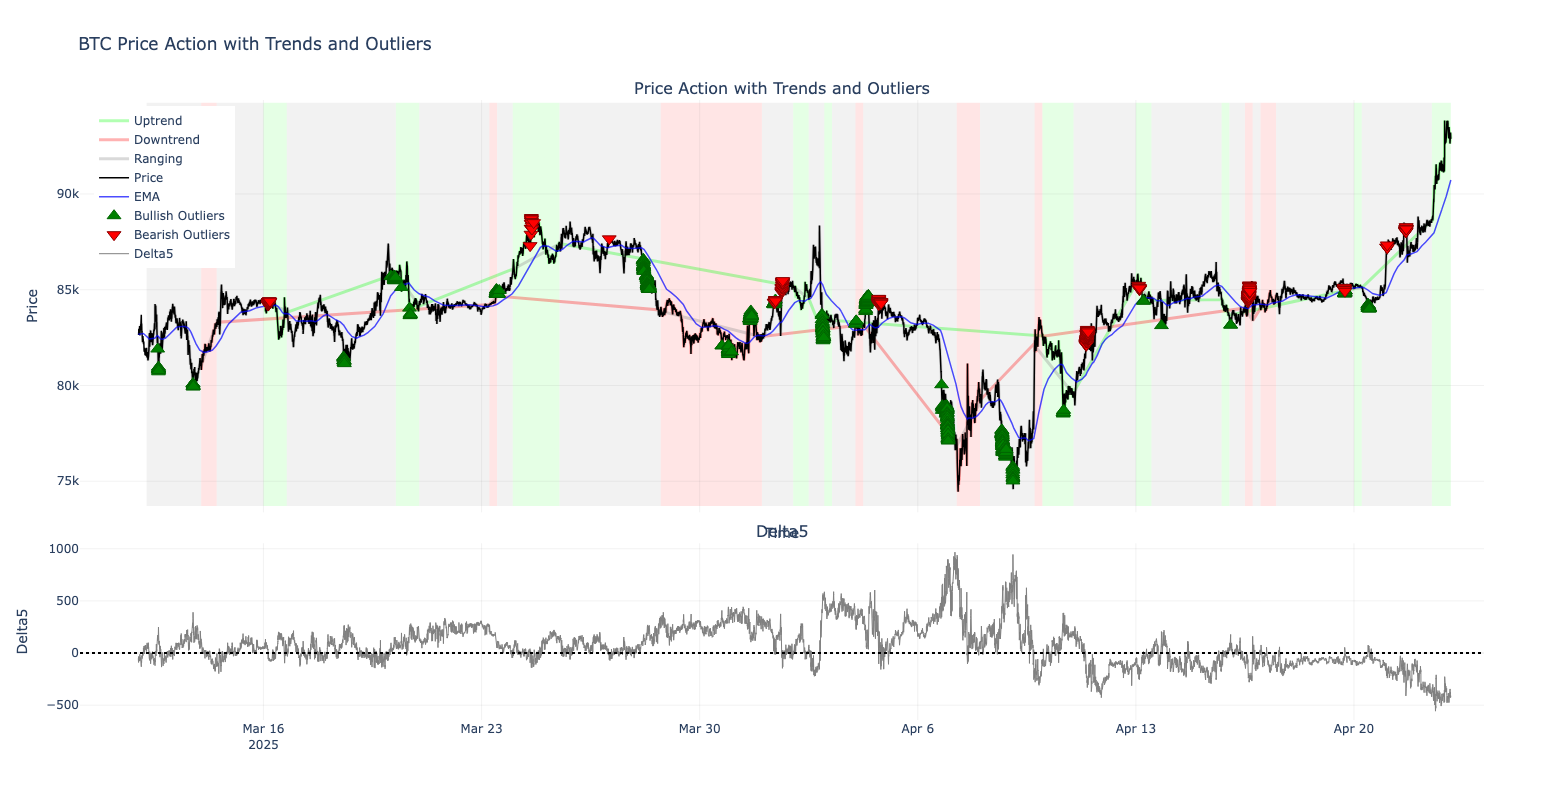
\includegraphics[width=\textwidth]{imgs/v2_plotting my idea.png}
  \caption{Visualization of $\Delta_t$ outliers and swing points}
\end{figure}

After plotting different kind of parts of Timeseries Data sets I created I was pretty sure that somewhere I would be finding an edge since the outliers often where at good entry points for a strategy. Only problem was I wasn't able to get any statistical proof ot this.
After finding a Github Repo which used Vectorbt to test 1000 strategies at the same time I tried a similar approach and tested different conditions to see if there was some kind of edge.









\subsection*{Monte Carlo Testing}

First of I have to explain how I search for a strategy and how it nearly killed my computer. 
We start by defining a different kind of sample sizes of all the $\Delta_t$ outliers time periods after the outlier detection. 
We want to know the return after our condition meets and then check in after $z$ minutes after that
\begin{verbatim}
  sampling_percentages = [0.1, 0.2, 0.6, 0.8, 1.0]
  holding_periods = [60, 120, 240, 360]  
\end{verbatim}

The sampling percentage definies how many of the existing outliers we use and test the returns on. So let's say we have $x$ amount of $\Delta_t$ Outliers. We then randomly select $z$ \% amount of outliers and test the returns on them. We do this 1000 times and then take the average return of all the 1000 tests.
The second step is to test each sampling percentage on the different holding periods. So let's say we have a sampling percentage of $z$ \% and a holding period of $y$ minutes. We then take the $z$ \% amount of outliers and test the returns on them after $y$ minutes. This test is basically copied from the Vectorbt Github Respository. I just changed the code to fit my needs and added some extra information returns. My code gives back the average return, the Sharpe, expectancy and mean Z-Score.

\begin{itemize}
  \item \textbf{Sharpe Ratio}: The Sharpe ratio is a measure of the risk-adjusted return of a strategy. It is calculated by dividing the average return of the strategy by the standard deviation of the returns.
  \item Calculated by $\frac{\overline{r}}{\sigma}$ Where $\overline{r}$ is the average return and $\sigma$ is the standard deviation of the returns.
  \item \textbf{Expectancy}: The expectancy is a measure of the profitability of a strategy. It is calculated by dividing the average return of the strategy by the average loss of the strategy.
  \item Calculated by $\frac{\overline{r}}{\overline{l}}$ Where $\overline{r}$ is the average return and $\overline{l}$ is the average loss.
  \item \textbf{Mean Z-Score}: The mean Z-Score is a measure of the average Z-Score of the strategy. It is calculated by taking the average of the Z-Scores of the strategy.
  \item Calculated by $\frac{1}{n}\sum_{i=1}^{n} z_i$ Where $z_i$ is the Z-Score of the strategy at time $i$ and $n$ is the number of Z-Scores.
  \item \textbf{Average Return}: The average return is a measure of the average return of the strategy. It is calculated by taking the average of the returns of the strategy.
  \item Calculated by $\frac{1}{n}\sum_{i=1}^{n} r_i$ Where $r_i$ is the return of the strategy at time $i$ and $n$ is the number of returns.



\end{itemize}



Now it is time to test some strategies. The first strategy I want to test is pretty intuitive. Measure the average return of bullish outliers inside of an uptrend.

\begin{list}{label}{spacing}
  \item A outlier is bullish if the the orderbook $\Delta_t$ is two standard deviations above the mean of the last 1440 $\Delta_t$ values and bearish if it is two standard deviations below the mean of the last 1440 $\Delta_t$ values.

\end{list}

Now when we backtest a strategy we have to have a few things in mind. First of all we are backtesting on on historical data and if we just use different kind of entry conditions we might just change the entry conditions till we have a good end results. This would be overfitting and not work on future data. 
In order to prevent overfitting we have to use a holdout sample. I have one dataset on which we test our entry conditions to see if they even have potential. 



\begin{table}[H]
  \centering
  \caption{Worth a out of sample test}
  \label{tab:strategy_results}
  \begin{tabular}{@{}lrr@{}}
    \toprule
      Sharpe Ratio &  Average Return  \\
    \midrule
      1.5 & 0.005 \\
    \bottomrule
  \end{tabular}
\end{table}

If these conditions are met for a condition I test on some out of sample data. (Out of sample data just means that we test on new data)
Most of the time things end up not even passing the first out of sample test and lose their potential instantly. If not I have another out of sample test and if that one is passed we are ready to do some more monte carlo testing and look how potential equity curves look like.
And to make things even worse we can assume that the sharpen ratio will decrease by atleast 20\% compared to the backtest simulation.




\newpage
\begin{figure}[H]
  \centering
  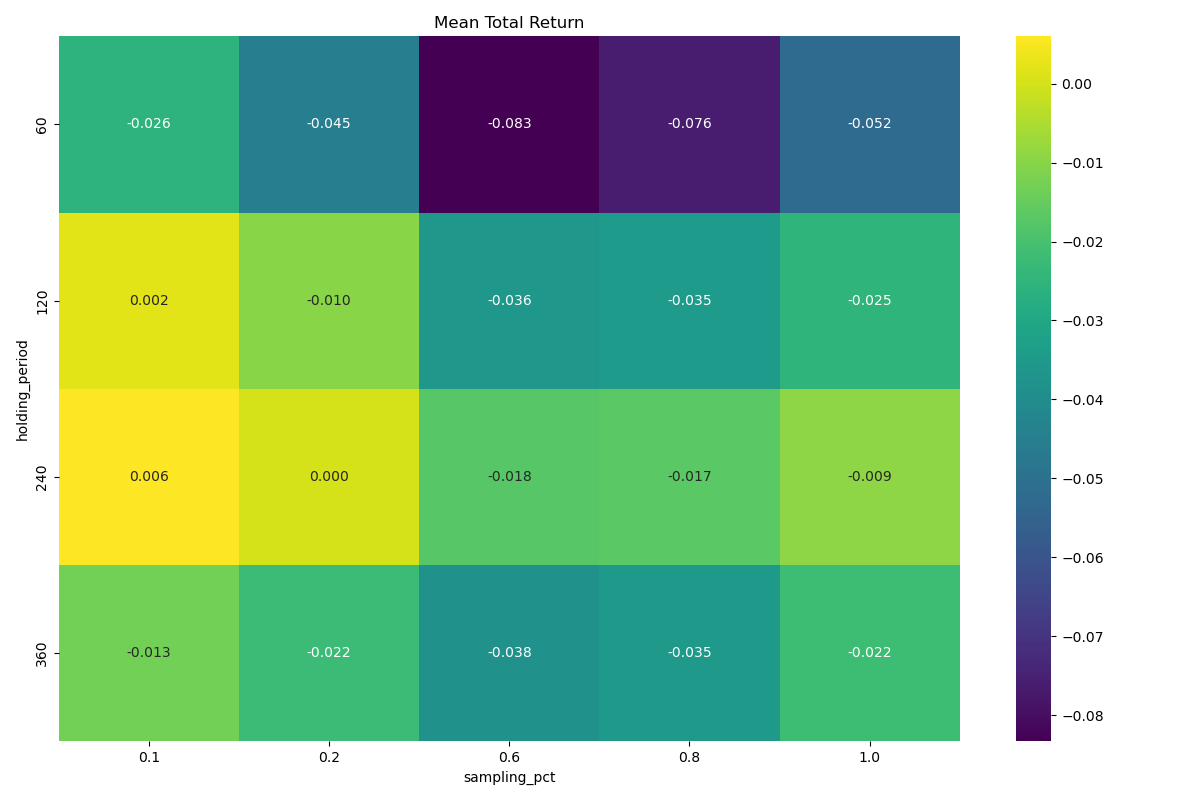
\includegraphics[width=\textwidth]{imgs/Bullish_outliers_inside_of_uptrend.png}
  \caption{Equity Curve of the strategy}
\end{figure}





\newpage
\section*{Developing a strategy}


\newpage
\section*{sources}
\subsection*{\href{https://x.com/HangukQuant/status/1930603876069335120}{How good or random is your trading}}
\subsection*{\href{https://github.com/polakowo/vectorbt}{Testing 1000 strategies at the same time (via Monte Carlo)}}
\subsection*{\href{https://x.com/abetrade/status/1941613701150188008}{ A lot of my ideas come from thiy guys Tweets, to research into this}}



\newpage



\end{document}